% !TEX program = lualatex
\documentclass[10pt,aspectratio=169]{beamer}

% =======================
%  FUENTE (Times New Roman)
% =======================
\usepackage{fontspec}
\IfFontExistsTF{Times New Roman}{\setmainfont{Times New Roman}}{\setmainfont{TeX Gyre Termes}}

% =======================
%  PAQUETES
% =======================
\usepackage{graphicx}
\usepackage{tikz}
\usepackage{ragged2e}
\usepackage{microtype}
%\usepackage{enumitem}
%\setlist[itemize]{nosep,leftmargin=1.2em}
%\setlist[enumerate]{nosep,leftmargin=1.2em}

% =======================
%  COLORES (paleta)
% =======================
\definecolor{FAMAFBlue}{RGB}{79,140,177}     % #4F8CB1
\definecolor{FAMAFBlue2}{RGB}{108,194,234}   % #6CC2EA
\definecolor{FAMAFBlue3}{RGB}{153,214,239}   % #99D6EF
\definecolor{FAMAFBlueDark}{RGB}{59,105,132} % #3B6984
\definecolor{FAMAFGray}{RGB}{245,248,250}

% =======================
%  AJUSTES DE FORMATO
% =======================
\setbeamercolor{normal text}{fg=black,bg=white}
\setbeamertemplate{navigation symbols}{}
\linespread{1.0}
\setlength{\parskip}{0pt}

% Mejor para slides (entra más y se ve limpio)
\AtBeginEnvironment{frame}{\raggedright}

% Márgenes del área de texto (controlá todo desde acá)
\setbeamersize{text margin left=0.8cm, text margin right=0.5cm}

% =======================
%  LISTAS (itemize) - visibles y compactas
% =======================
% Símbolos (podés cambiar fácilmente acá)
\setbeamertemplate{itemize item}{\raise0.15ex\hbox{\large\textbullet}}
\setbeamertemplate{itemize subitem}{\raise0.10ex\hbox{\normalsize\textopenbullet}}
\setbeamertemplate{itemize subsubitem}{\raise0.10ex\hbox{\scriptsize$\diamond$}}

% Colores de bullets
\setbeamercolor{itemize item}{fg=FAMAFBlueDark}
\setbeamercolor{itemize subitem}{fg=FAMAFBlueDark}
\setbeamercolor{itemize subsubitem}{fg=FAMAFBlueDark}

% Compactación vertical beamer-friendly
\setbeamertemplate{itemize/enumerate body begin}{\vspace{-2pt}}
\setbeamertemplate{itemize/enumerate body end}{\vspace{-2pt}}

% Sangrías: NO uses \leftmargini acá (Beamer lo gestiona por templates/márgenes)
% Si querés más/menos sangría de lista, lo mejor es tocar text margin left/right arriba.

% =======================
%  BLOQUES (compactos)
% =======================
\setbeamertemplate{blocks}[rounded][shadow=false]
\setbeamerfont{block title}{size=\normalsize,series=\bfseries}
\setbeamerfont{block body}{size=\normalsize}
\addtobeamertemplate{block begin}{}{\vspace{-2pt}}
\addtobeamertemplate{block end}{}{\vspace{-2pt}}

% =======================
%  HEAD/FOOT
% =======================
\setbeamercolor{section in head/foot}{bg=white, fg=FAMAFBlueDark}

% =======================
%  LOGO (único)
% =======================
\newcommand{\FamafLogo}{./attatchments/Logo_FAMAF_UNC_negro.png}
\newcommand{\LogoHeight}{1.10cm}      % tamaño en contenido (abajo derecha)
\newcommand{\LogoHeightTitle}{1.70cm} % tamaño en portada (centrado)

\newcommand{\LogoGraphic}[1]{%
  \includegraphics[height=#1,keepaspectratio]{\FamafLogo}%
}

% Flag para mostrar logo overlay en contenido
\newif\ifshowcontentlogo
\showcontentlogotrue

% Logo en contenido: abajo a la derecha (overlay)
\newcommand{\PlaceLogoBottomRight}{%
  \begin{tikzpicture}[remember picture,overlay]
    % Si el logo pisa el borde inferior, subí yshift (ej: 0.35cm o 0.40cm)
    \node[anchor=south east,inner sep=0pt] at ([xshift=-0.35cm,yshift=0.30cm]current page.south east)
    {\LogoGraphic{\LogoHeight}};
  \end{tikzpicture}%
}

% Hook automático: mete logo overlay SOLO cuando el flag está activo
\addtobeamertemplate{background canvas}{}{%
  \ifshowcontentlogo
    \PlaceLogoBottomRight
  \fi
}

% =======================
%  ESTILO / TÍTULOS
% =======================
\setbeamercolor{title}{fg=FAMAFBlueDark}
\setbeamercolor{frametitle}{fg=FAMAFBlueDark}
\setbeamerfont{title}{series=\bfseries,size=\Large}
\setbeamerfont{frametitle}{series=\bfseries,size=\normalsize}

% Barra superior sutil
\setbeamertemplate{headline}{
  \begin{beamercolorbox}[
    wd=\paperwidth,
    ht=0.9cm,
    dp=0.25cm,
    leftskip=0.4cm,
    rightskip=0.4cm
  ]{section in head/foot}

    {\small\bfseries\color{FAMAFBlueDark}
      \insertsectionhead
    }

    \vspace{0.1cm}
    \color{FAMAFBlue}\rule{\paperwidth}{0.6pt}
  \end{beamercolorbox}
}

\setbeamertemplate{frametitle}{
  \vspace{-0.20cm} % sube el título (ajustable)
  \begin{beamercolorbox}[
    wd=\paperwidth,
    ht=0.70cm,      % altura fija más chica
    dp=0.10cm,      % profundidad (baja el "aire" debajo)
    leftskip=0.8cm, % alineado con tus márgenes
    rightskip=0.5cm
  ]{frametitle}
    \usebeamerfont{frametitle}\insertframetitle
  \end{beamercolorbox}
  \vspace{-0.15cm} % recorta el espacio entre título y contenido
}

% Bloques
\setbeamercolor{block title}{fg=black,bg=FAMAFBlue3}
\setbeamercolor{block body}{fg=black,bg=FAMAFGray}

\newcommand{\BulletsOff}{%
  \setbeamertemplate{itemize item}{}%
  \setbeamertemplate{itemize subitem}{}%
  \setbeamertemplate{itemize subsubitem}{}%
}

% =======================
%  METADATOS
% =======================
\title[Presentación]{Redes Neuronales biologicamente inspiradas aplicadas al aprendizaje por refuerzo profundo}
\author{Adolfo Banchio}
\date{\today}

% Agenda por secciones (opcional)
%\AtBeginSection[]{
%  \begin{frame}{}
%    \tableofcontents[currentsection]
%  \end{frame}
%}

% =======================
%  DOCUMENTO
% =======================

\begin{document}

% -------------------------------------------------
% 1) PORTADA (centrada + fondo azul oscuro + logo centrado en el pie)
% -------------------------------------------------
{
\showcontentlogofalse % desactiva el logo overlay SOLO en la portada
\setbeamercolor{background canvas}{bg=FAMAFBlueDark}

\begin{frame}[plain]
  \vfill
  \centering
  {\usebeamerfont{title}\color{white}\inserttitle\par}
  \vspace{0.5cm}
  {\large\color{white}\insertauthor\par}
  \vspace{0.2cm}
  {\normalsize\color{white}\insertdate\par}
  \vfill

  {\small\color{white}Director: Dr. Martín A. Domínguez\par}
  {\small\color{white}Facultad de Matemática, Astronomía, Física y Computación (FaMAF)\par}

  % Logo centrado en el pie (portada)
  \LogoGraphic{\LogoHeightTitle}
  \vspace{0.15cm}

\end{frame}
}

% -------------------------------------------------
% 2) AGENDA GENERAL (logo abajo derecha)
% -------------------------------------------------
\begin{frame}{Estructura de la presentación}
  \tableofcontents
\end{frame}

% -------------------------------------------------
% SECCIONES DE EJEMPLO
% -------------------------------------------------
\section{Motivación}

\begin{frame}{Inteligencia Artificial y ML}
  \begin{itemize}
    \item Busqueda de \textbf{agentes} capaces de tomar la decision correcta en funcion de la información disponible.
  \end{itemize}

  \begin{block}{Aprendizaje automático (\textbf{Machine Learning})}
    Un programa de computadora aprende de la experiencia E con repecto a alguna clase de tareas T y una medida de desempeño P, si su desempeño en tareas de T, medidio por P, mejora con la experiencia E.
  \end{block}
  Segun el tipo de experiencia y medida de desempeño, se divide en:
  
    \begin{itemize}
      \item Aprendizaje supervisado
      \item Aprendizaje no supervisado
      \item \textbf{Aprendizaje por refuerzo}
    \end{itemize}
\end{frame}

\begin{frame}{Aprendizaje por Refuerzo (RL)}
  \begin{columns}[T,onlytextwidth]

    % ---- Columna izquierda: texto ----
    \column{0.50\textwidth}
    Un agente interactúa con un entorno dinámico donde:
    \begin{itemize}
        \item Observa estados $s_t$
        \item Ejecuta acciones $a_t$
        \item Recibe recompensas $r_{t+1}$
    \end{itemize}

    \vspace{0.2cm}
    Con el objetivo de maximizar la recompensa final acumulada:
    \[
    \max_\pi \ \mathbb{E}[R]
    \]

    Principales desafíos:
    \begin{itemize}
        \item Problema de asignación de crédito
        \item Exploración vs explotación
        \item Retroalimentación escasa y diferida
    \end{itemize}

    % ---- Columna derecha: imagen ----
    \column{0.50\textwidth}
    \begin{center}
      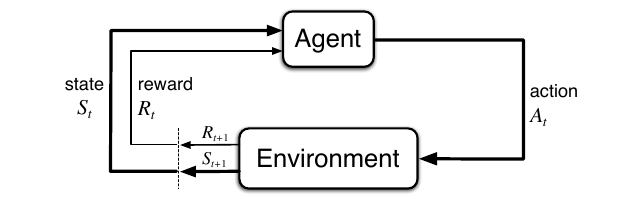
\includegraphics[
        width=\linewidth,
        height=0.75\textheight,
        keepaspectratio
      ]{./attatchments/interaccion_rl.png}
    \end{center}
  \end{columns}
\end{frame}

\begin{frame}{Redes Neuronales}
  \begin{columns}[T,onlytextwidth]

    % ---- Columna izquierda: texto ----
    \column{0.40\textwidth}
      \begin{itemize}
        \item Comunmente utilizadas como aproximadores de funciones universales.
        \item Se entrenan mediante metodos basados en el \textbf{descenso por el gradiente}. 
      \end{itemize}
      \vspace{0.4cm}
      \[
        \theta \leftarrow \theta - \alpha \nabla_\theta L(\theta)
      \]

    % ---- Columna derecha: imagen ----
    \column{0.60\textwidth}
      \begin{center}
        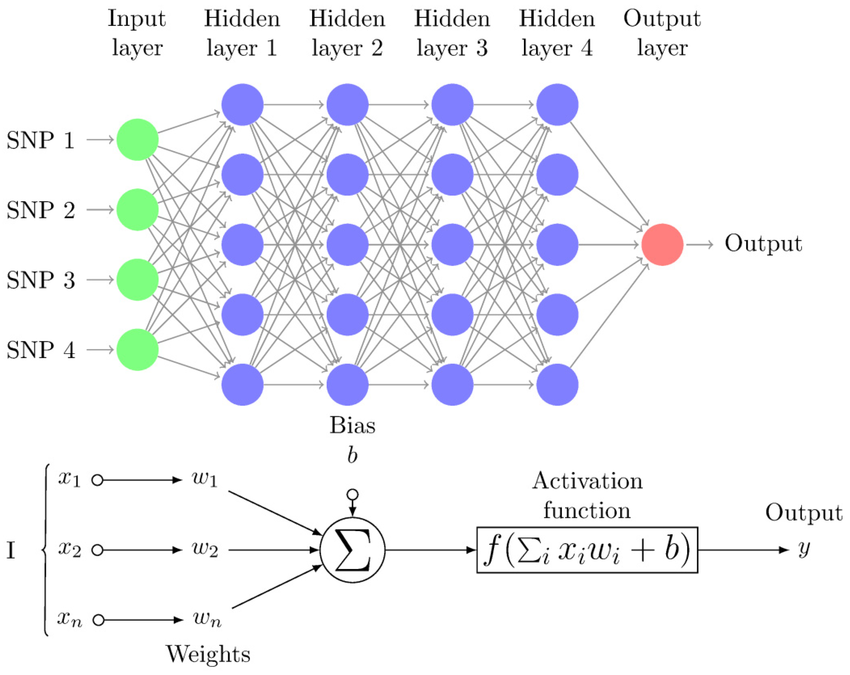
\includegraphics[
          width=\linewidth,
          height=0.75\textheight,
          keepaspectratio
        ]{./attatchments/mlp.png}
      \end{center}
  \end{columns}
\end{frame}

\begin{frame}{Antecedentes y objetivo}
  \pause
  
  Trabajos anteriores lograron:
  \begin{itemize}
      \item Integrar una \textbf{arquitectura neuronal bioinspirada} (Tap Withdrawal Circuit de \textit{C. elegans}) en el marco del aprendizaje por refuerzo.
      \item Plantear nuevos modelos neuronales (\textbf{modelo Fiuri}) y compararlos con modelos estándar (IandF, Izikievich).
      \item Utilizar metodos de entrenamiento alternativos al descenso por el gradiente (Optimizacion bayesiana, algoritmos geneticos y busquedas aleatoreas).
  \end{itemize}
  
  \pause
  \begin{block}{Pregunta central}
  ¿Puede una arquitectura neuronal biológicamente inspirada (TWC + FIU) entrenarse con métodos basados en gradiente y tener desempeño competitivo?
  \end{block}
\end{frame}


\section{El Agente Bioinspirado}

\begin{frame}{Dinamica Neuronal FIU}
  \begin{columns}[T,onlytextwidth]
    \column{0.50\textwidth}

    % Compactar SOLO las ecuaciones (no toda la slide)
    {\small
    \setlength{\abovedisplayskip}{2pt}
    \setlength{\belowdisplayskip}{2pt}
    \setlength{\jot}{2pt}

    \begin{equation*}
      \begin{aligned}
        S_n &= E_n + \sum_{j=1}^{m} I_{in}^{j}
      \end{aligned}
    \end{equation*}

    \begin{equation*}
      O_n =
      \begin{cases}
        S_n - T_n, & \text{si } S_n > T_n \\
        0,         & \text{en otro caso}
      \end{cases}
    \end{equation*}

    \begin{equation*}
      E_n =
      \begin{cases}
        S_n - T_n, & \text{si } S_n > T_n \\
        E_n - d_n, & \text{si } S_n \le T_n \ \land\  S_n = E_n \\
        S_n,       & \text{en otro caso}
      \end{cases}
    \end{equation*}

    \begin{equation*}
      I_{in}^{j} =
      \begin{cases}
        \ \omega_j O_j, & \text{gap junc. y } O_j \ge E_n \\
        -\omega_j O_j,  & \text{gap junc. y } O_j < E_n \\
        \ \omega_j O_j, & \text{exc. química} \\
        -\omega_j O_j,  & \text{inh. química}
      \end{cases}
    \end{equation*}
    } % end \small

    \column{0.50\textwidth}
    TODO: Ilustracion de una neurona o como fue implementada (placeholder)
  \end{columns}
\end{frame}

\begin{frame}{La arquitectura TWC}
  \centering
    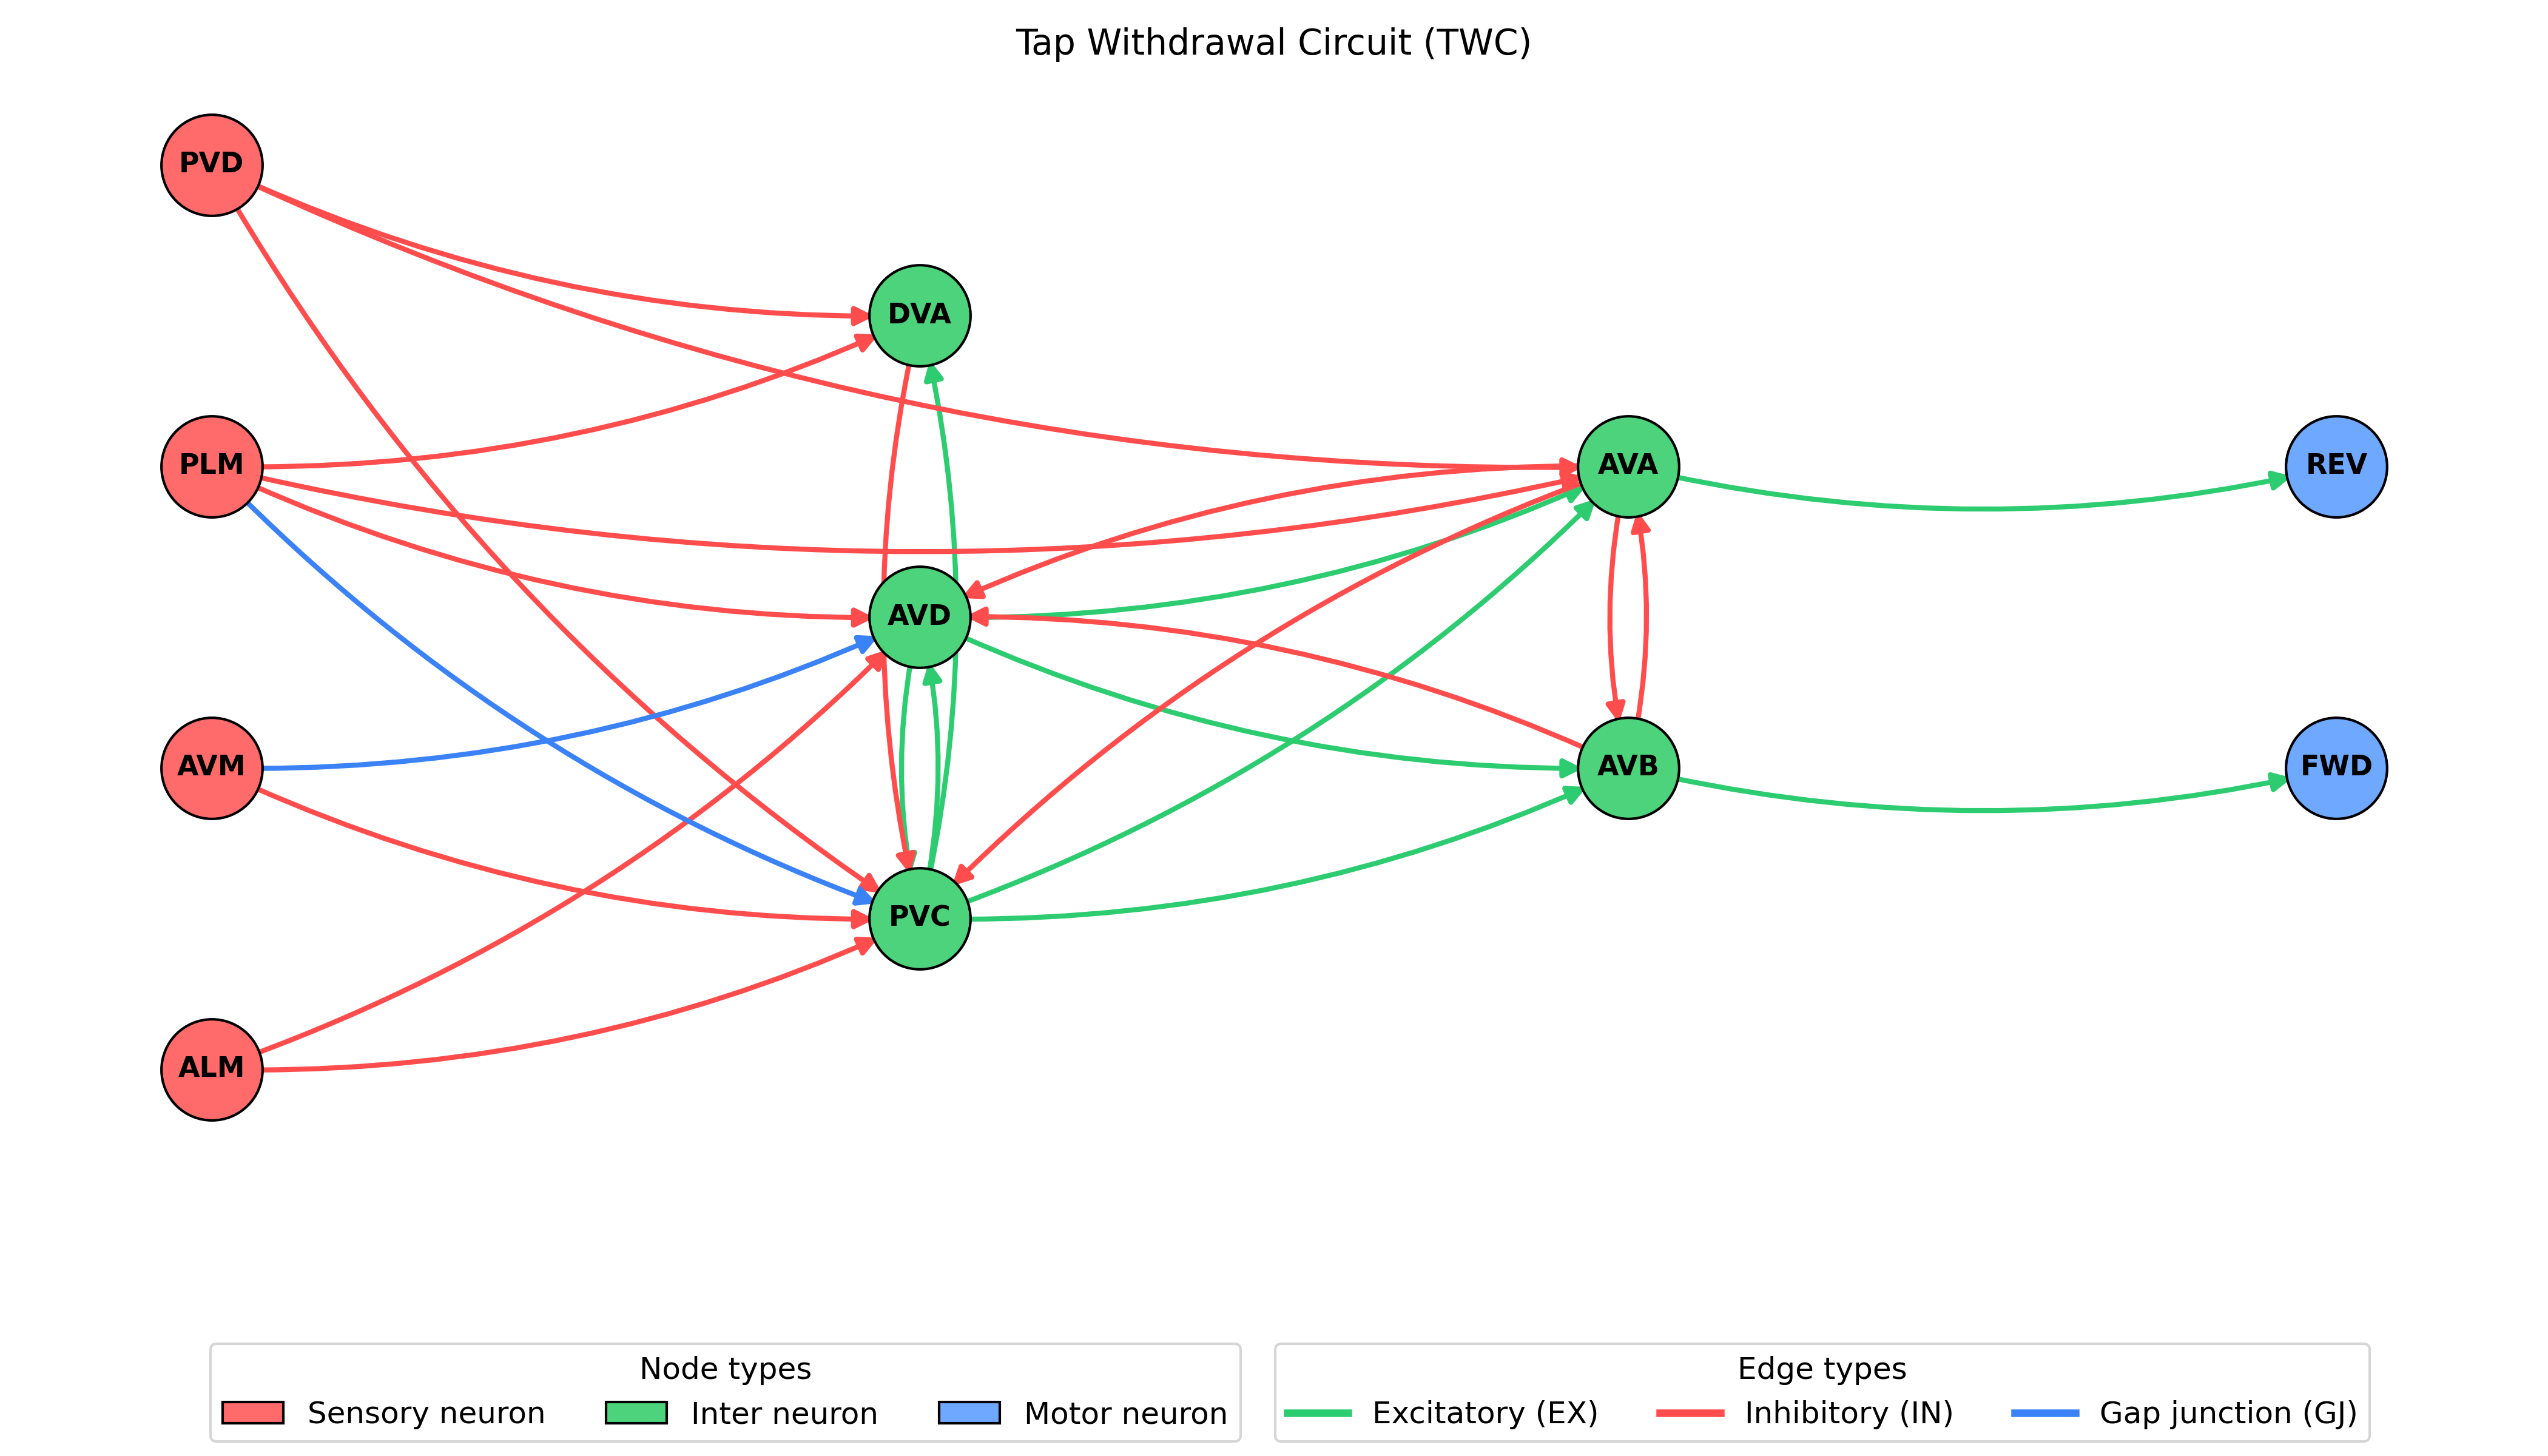
\includegraphics[
      width=\linewidth,
      height=0.82\textheight,
      keepaspectratio
    ]{./attatchments/twc.png}
\end{frame}


% -------------------------------------------------
% 3) DIAPOSITIVA DE CONTENIDO (logo abajo derecha)
% -------------------------------------------------
\begin{frame}{Título de la diapositiva de contenido}
  \begin{block}{Idea principal / Resultado}
    Texto placeholder para explicar la idea principal. Podés escribir 2--4 líneas
    sin que quede demasiado aire.
  \end{block}

  \vspace{0.25cm}

  \textbf{Puntos clave:}
  \begin{itemize}
    \item Punto 1 (placeholder).
    \item Punto 2 (placeholder).
    \item Punto 3 (placeholder).
    \item hola
  \end{itemize}

  \vspace{0.15cm}

  \textbf{Figura (placeholder):}
  \begin{center}
    \fbox{
      \parbox{0.75\linewidth}
      {
        \centering 
          \begin{figure}
            
\includegraphics[width=0.8\textwidth]{./attatchments/unc3_a.jpg}
            \caption{Figura placeholder. Reemplazá esto con tu propia figura.}
          \end{figure}
      }
      }
  \end{center}
\end{frame}

\begin{frame}{Título de la diapositiva con imagen}
  \begin{columns}[T,onlytextwidth]

    % ---- Columna izquierda: texto ----
    \column{0.45\textwidth}
    \textbf{Idea principal}

    Texto introductorio breve que contextualiza la imagen. Idealmente 2–3 líneas
    para no desperdiciar espacio vertical.

    \vspace{0.2cm}

    \begin{itemize}
      \item Punto clave 1 relacionado con la imagen.
      \item Punto clave 2 (explicación breve).
      \item Punto clave 3 si es necesario.
    \end{itemize}

    \vspace{0.15cm}

    Texto final opcional para cerrar la idea o remarcar una conclusión.

    % ---- Columna derecha: imagen ----
    \column{0.55\textwidth}
    \begin{center}
      
\includegraphics[
        width=\linewidth,
        height=0.75\textheight,
        keepaspectratio
      ]{./attatchments/unc3_a.jpg}
    \end{center}

  \end{columns}
\end{frame}


% -------------------------------------------------
% 4) AGRADECIMIENTOS (logo abajo derecha)
% -------------------------------------------------
{
\setbeamercolor{background canvas}{bg=FAMAFBlueDark}
\showcontentlogofalse 

\begin{frame}[plain]
  \vfill
  \centering
  {\Huge\bfseries\color{white}¡Muchas Gracias!}
  \vfill

  {\Large\color{white}¿Preguntas?}
  \vfill

  \LogoGraphic{\LogoHeightTitle}
\end{frame}
}

\end{document}